\documentclass[lettersize,journal]{IEEEtran}
\usepackage{amsmath,amsfonts}
\usepackage{algorithmic}
\usepackage{algorithm}
\usepackage{array}
\usepackage[caption=false,font=normalsize,labelfont=sf,textfont=sf]{subfig}
\usepackage{textcomp}
\usepackage{stfloats}
\usepackage{url}
\usepackage{verbatim}
\usepackage{graphicx}
\usepackage{cite}
\usepackage{booktabs}
\hyphenation{op-tical net-works semi-conduc-tor IEEE-Xplore}

\begin{document}

\title{Precise Visual Servoing for Suction Cup Grippers Using Foundation Model Segmentation}

\author{Akanksha Singal,~\IEEEmembership{Robotics Institute,~CMU}
\thanks{This work was carried out as part of an independent study in the Master of Science
in Computer Vision program at Carnegie Mellon University's Robotics Institute under the
supervision of Prof.\ Jeffrey Ichnowski, Momentum Robotics Lab.}}

\markboth{IEEE Robotics and Automation Letters}%
{Singal: Precise Visual Servoing for Suction Cup Grippers}

\maketitle

% =========================================================================
\begin{abstract}
Reliable suction-cup grasping of boxes in unstructured environments requires a
robot to locate a valid surface patch and close the distance to it with
millimetre-level precision.  We present a hierarchical visual servoing system
for a 6-DOF manipulator that requires only a single reference image of the
target object and no task-specific retraining.  During the far-range
approach, the target is detected and segmented every frame using
SAM3 open-vocabulary segmentation, guided by cosine similarity to the
reference image.  As the end effector closes in and the object begins to
exit the camera field of view, the system transitions to a multi-signal
fusion estimator that combines a locked 3-D projection, CoTracker3 point
tracking, a SAM2 watchdog, and DINOv2 feature matching via a
Weiszfeld weighted geometric median.  A final RANSAC plane fit on
stereo depth data drives the approach direction to align with the surface
normal of the target face.  We describe the full pipeline, its control
law and online Jacobian calibration, and compare four perception
architectures (SAM3, GroundingDINO with SAM2, OWLv2 with SAM2, and
DINOv2 feature matching) in an ablation study.  A pilot trial on a
protein-bar box demonstrates the system executing a 296\,mm forward
approach while maintaining SAM3 detection confidence above 0.94 throughout.
\end{abstract}

\begin{IEEEkeywords}
Visual servoing, suction grasping, image-based visual servoing, foundation models,
SAM3, object segmentation, xArm, ZED Mini.
\end{IEEEkeywords}


% =========================================================================
\section{Introduction}
\label{sec:intro}

Autonomous suction-cup grasping is a critical capability for warehouse
automation, logistics handling, and unstructured pick-and-place.  A suction
gripper requires the end effector (EE) to make contact with a flat face of
the target object within a tight positional and angular tolerance: lateral
placement errors exceeding a few millimetres or approach angles deviating
more than a few degrees from the surface normal risk a failed vacuum seal.
Achieving this precision from a single monocular or stereo camera mounted
on the EE is the central challenge addressed in this work.

Image-based visual servoing (IBVS) is a natural fit for this task: it uses
continuous visual feedback to reduce the gap between the observed target
and the desired configuration, avoiding the need for an accurate world model
or precise hand-eye calibration during the servoing phase.  Classical IBVS
formulations drive image-plane feature errors to zero via a learned or
analytically derived interaction matrix.  However, classical feature
extractors are brittle to changes in object appearance, viewpoint, background
clutter, or illumination, making them poorly suited to unstructured deployment
without task-specific calibration.

Modern vision foundation models---large neural networks pretrained on
internet-scale data---offer a promising path to appearance-robust perception
without retraining.  SAM3 (Segment Anything Model 3) performs open-vocabulary
detection and instance segmentation in a single forward pass from a text
prompt.  GroundingDINO and OWLv2 provide open-vocabulary bounding-box
detection that can be further refined with a promptable segmentation network
such as SAM2.  DINOv2 produces dense patch-level feature representations
that support bidirectional nearest-neighbour matching across viewpoints.
CoTracker3 propagates a set of query points through video using a
transformer-based online tracker.  By combining these models, it becomes
possible to build a visual servoing pipeline that requires only a single
reference image of the target object and generalises across box types,
backgrounds, and clutter without additional data collection.

However, deploying such a pipeline on a real robot exposes a structural
challenge that does not arise in static benchmarks: as the EE approaches the
target, the object grows larger in the image and eventually exits the field
of view of the camera.  Under this partial-framing condition, a mask-based
centroid estimate drifts toward the visible portion of the object rather than
the true face centre, corrupting the error signal.  A robust approach must
detect this onset and transition to a signal source that remains well-defined
even when the object boundary is no longer fully contained in the image.

This paper makes the following contributions:
\begin{enumerate}
  \item A complete hierarchical visual servoing pipeline for suction-cup
        grasping that operates from a single reference image without
        task-specific retraining, structured as a four-state machine
        (\textsc{far} $\to$ \textsc{lock} $\to$ \textsc{near} $\to$
        \textsc{terminal}).
  \item A multi-signal fusion estimator for the close-range phase that
        combines four heterogeneous signal sources---locked 3-D reprojection,
        CoTracker3 point tracking, SAM2 video segmentation, and DINOv2
        feature matching---via a Weiszfeld weighted geometric median, with
        an explicit watchdog to detect signal divergence.
  \item An online Jacobian calibration procedure that estimates the pixel
        response to lateral EE translations via optical flow, enabling
        correct IBVS control without manual camera--robot calibration.
  \item A RANSAC-based surface normal estimator that quantifies the tilt
        of the target face relative to the approach axis and provides the
        angular correction needed for contact alignment.
  \item A quantitative comparison of four perception architectures in an
        ablation study spanning five box types, four environmental
        configurations, and three starting poses.
\end{enumerate}

The remainder of this paper is organised as follows.
Section~\ref{sec:related} reviews related work.
Section~\ref{sec:learning} describes the earlier learning-based approach,
its training setup, and the sim-to-real failure modes that motivated the
present design.
Section~\ref{sec:system} describes the hardware and high-level system design.
Section~\ref{sec:method} details the control law, Jacobian calibration,
far-range segmentation pipeline, and close-range fusion estimator.
Section~\ref{sec:baselines} describes the baseline perception variants used
in the ablation study.
Section~\ref{sec:experiments} presents the experimental protocol and results.
Section~\ref{sec:discussion} discusses open issues and limitations.
Section~\ref{sec:conclusion} concludes.


% =========================================================================
\section{Related Work}
\label{sec:related}

\subsection{Image-Based Visual Servoing}

Image-based visual servoing (IBVS) was formalised by Espiau
\emph{et al.}~\cite{espiau1992new} and reviewed comprehensively by Chaumette
and Hutchinson~\cite{chaumette2006visual,chaumette2007visual}.  Classical
IBVS minimises the error between observed and desired image features
(point coordinates, line moments, region centroids) via the image Jacobian
(interaction matrix).  The interaction matrix is either derived analytically
from 3-D object models or estimated online from small EE perturbations.
For unknown objects and uncalibrated cameras, brute-force online estimation
of the Jacobian through probing motions was explored early in the
literature~\cite{piepmeier2004uncalibrated}.

A key limitation of classical IBVS is sensitivity to feature extraction
failures under clutter, illumination change, or large viewpoint variation.
Approaches that replace hand-crafted features with deep representations have
demonstrated improved robustness.  Bateux and
Marchand~\cite{bateux2017training} and Saxena \emph{et al.}~\cite{saxena2017neural}
showed that neural network features can serve as stable visual error
signals.  More recently, work combining learned dense descriptors with
classical servoing loops~\cite{lampe2023learning} has shown generalisation
across object categories.

\subsection{Foundation Models for Robotic Manipulation}

Large pretrained vision models have rapidly expanded the capabilities of
zero-shot and one-shot robot perception.  The Segment Anything Model
(SAM)~\cite{kirillov2023segment} and its video-aware successor
SAM2~\cite{ravi2024sam2} provide high-quality instance masks from minimal
prompts (bounding boxes, points, or text).  SAM3 extends this with
Promptable Concept Segmentation (PCS), which jointly detects and segments
all instances of a concept from a text query in a single pass, eliminating
the two-stage detect-then-segment bottleneck.

GroundingDINO~\cite{liu2023grounding} combines a Transformer-based object
detector with grounded language understanding, achieving strong
open-vocabulary detection across object categories.  OWLv2~\cite{minderer2023scaling}
follows a similar approach and additionally supports an image-guided query
mode in which a reference crop is passed alongside the text prompt to bias
detection toward visually similar instances.  These detectors have been
integrated into manipulation pipelines for one-shot grasping~\cite{liu2024graspgdino}
and affordance prediction~\cite{tang2023taskgrasp}.

DINOv2~\cite{oquab2023dinov2} produces powerful patch-level feature
representations without supervision.  Bidirectional best-buddy
matching~\cite{amir2022deep} on DINOv2 features has been shown to yield
accurate keypoint correspondences across large viewpoint and appearance
changes, making it attractive for reference-guided object retrieval.

CoTracker3~\cite{karaev2024cotracker3} tracks arbitrary query points through
video by jointly predicting their positions and visibility scores from a
sliding window of frames.  Its online mode enables deployment in streaming
settings without buffering a full video.

\subsection{Visual Servoing Under Partial Occlusion and Close Approach}

When a camera-in-hand system approaches a planar target, the object
eventually exceeds the camera's field of view.  Maintaining a valid control
signal under this condition has received limited attention in the IBVS
literature.  Yoshimi and Allen~\cite{yoshimi1994active} noted the problem in
the context of grasping and proposed switching to contact sensing near the
target.  More recent work on hand-guiding and teleoperation has used
point-cloud or tactile feedback as a late-stage signal.  Our multi-signal
fusion architecture addresses this gap by maintaining four independent
centroid estimates and fusing them through a robust aggregation rule,
allowing the pipeline to continue functioning after any individual signal
becomes unreliable.

\subsection{Suction Grasping}

Suction cup grasping requires estimating a suitable contact patch on the
target surface.  Classical approaches fit planes or cylinders to point-cloud
data and score patches by contact area and surface
smoothness~\cite{mahler2017dex}.  Deep learning methods such as GQ-CNN and
Dex-Net~\cite{mahler2019learning} regress grasp quality from RGB-D input.
These approaches require training data and do not directly address the
problem of closing the distance to a chosen contact point with visual
feedback.  Our system focuses on the final-approach stage: given a detected
target, it drives the EE to the face centre using purely visual signals.


% =========================================================================
\section{Learning-Based Approach and Sim-to-Real Gap}
\label{sec:learning}

Before arriving at the foundation-model pipeline described in this paper,
a supervised learning approach was developed and evaluated.  This section
describes that effort, its training setup and architecture family, and the
specific failure modes that led to its abandonment in favour of the
zero-shot, foundation-model-based system.

\subsection{Problem Formulation}

The learning-based approach framed last-mile visual servoing as a supervised
regression problem.  Given one or two camera images captured by the
eye-in-hand ZED Mini, a neural network was trained to predict a 3-D servo
offset $(\Delta x, \Delta y, \Delta z)$ that would move the end effector
to the target grasp point.  The target offsets were expressed in metres,
with a lateral range of $\pm 0.30$\,m in each of the two lateral axes and
a depth range of $\pm 0.13$\,m along the forward axis.

Two input modalities were explored: a \emph{monocular} variant consuming
only the left camera frame, and a \emph{stereo} variant consuming both the
left and right frames of the ZED Mini simultaneously.

\subsection{Dataset Generation}

Training data were generated entirely in Isaac Sim, a physics-based
photorealistic simulator.  The simulated scene placed a box on a table
and rendered synthetic stereo image pairs from a virtual camera mounted
at the tool flange, varying the end-effector pose relative to the box
across a grid of offsets.  Each sample in the dataset consisted of a
left-right stereo image pair (stored as RGBA PNG files at $224 \times 224$
pixels) paired with the ground-truth 3-D servo offset extracted directly
from the simulator's scene graph.  The dataset was indexed via JSON
manifests containing the frame index and the corresponding offset label
for each key frame.

\subsection{Network Architectures}

Four model families were implemented and compared for both the stereo and
monocular input modes.

\textbf{Custom CNN.}
The baseline stereo model (\emph{DualStreamCNN}) used a shared
convolutional feature extractor applied independently to the left and right
images.  The extractor consisted of three stages of convolution, batch
normalisation, and rectified linear units, followed by adaptive average
pooling to a $1\times1$ feature map of 256 channels.  The resulting feature
vectors for both images were concatenated into a 512-dimensional
representation and passed through a three-layer fusion head predicting the
3-D offset.  The monocular counterpart (\emph{MonocularCNN}) used a single
stream producing a 256-dimensional vector fed directly into a regression
head of the same depth.

\textbf{Pretrained EfficientNet.}
A dual-stream variant replaced the custom backbone with a pretrained
EfficientNet-B0 feature extractor (1280-dimensional output per stream).
The left features, right features, and their element-wise difference were
concatenated into a 3840-dimensional vector before the regression head.
Early convolutional blocks (the first four MBConv stages) were frozen
during training to preserve low-level pretrained representations.

\textbf{Pretrained ResNet.}
A parallel variant used pretrained ResNet-18, ResNet-34, or ResNet-50 as
the backbone, producing 512- or 2048-dimensional feature vectors per
stream.  The same left-plus-right-plus-difference fusion strategy was
applied.

\textbf{Neural Circuit Policy head.}
A fourth variant replaced the fully connected regression head with a
Closed-form Continuous-time (CfC) neural network organised as a Neural
Circuit Policy (NCP) with an AutoNCP wiring.  The CNN backbone (five
convolutional layers producing a 128-dimensional feature vector per stream
after a fully connected projection) fed the concatenated features into the
NCP head as a single-step sequence, producing the 3-D offset as output.
The NCP head was intended to introduce biologically inspired, sparse
connectivity as an inductive bias for smooth control signals.

\subsection{Training Protocol}

All models were trained using the Adam optimiser with a learning rate of
$10^{-4}$ and a ReduceLROnPlateau scheduler (factor 0.5, patience 5
epochs).  Training ran for 100 epochs with batch size 4.  Input images
were resized to $224\times224$ and normalised using ImageNet channel
statistics.

The loss function was a weighted mean squared error in which each output
dimension was weighted inversely proportional to the square of its
physical range, so that the depth axis (range 0.13\,m) received
proportionally more gradient signal than the wider lateral axes (range
0.30\,m each):
\begin{equation}
  \mathcal{L} = \sum_{k \in \{x,y,z\}}
    \frac{w_k}{N} \sum_{i=1}^{N} (\hat{\delta}_k^{(i)} - \delta_k^{(i)})^2,
  \quad w_k = \frac{1/r_k^2}{\sum_j 1/r_j^2},
  \label{eq:wmsed}
\end{equation}
where $r_k$ is the physical range of axis $k$ and $\hat{\delta}_k^{(i)}$
is the predicted offset for sample $i$.

\subsection{Sim-to-Real Gap and Failure Modes}

Despite achieving low validation loss on held-out synthetic data, all
trained models failed to generalise to real robot operation.  The
failure can be attributed to a combination of the following sources of
sim-to-real gap.

\textbf{Visual domain shift.}
Isaac Sim renders photorealistic scenes but cannot reproduce the specific
optical properties of the ZED Mini: lens distortion, stereo rectification
artefacts, automatic exposure and white-balance variation, and the
characteristic noise pattern of the CMOS sensor.  The simulated images
had uniformly lit, shadow-free surfaces; real images had specular
highlights on box faces, cast shadows from the robot arm, and motion blur
from vibration during approach.  The convolutional feature extractors
trained exclusively on synthetic data encoded domain-specific texture
statistics that did not transfer to real sensor output.

\textbf{Object appearance generalisation.}
The synthetic dataset used a small set of simulated box geometries with
flat, uniformly coloured surfaces.  Real boxes carry printed graphics,
barcodes, and branding elements distributed unevenly across the visible
face.  Because the models received no reference image of the target and
had no mechanism for instance-level discrimination, they could not
distinguish the target box from distractors or from the background.

\textbf{Ground-truth label noise floor.}
In simulation, the servo offset label was exact.  In any real validation
attempt, ground-truth offset measurement required manually jogging the
end effector to the face centre, introducing a placement repeatability
error of approximately 3--5\,mm that the model had not been trained to
tolerate.

\textbf{Depth axis underrepresentation.}
The depth axis range ($\pm 0.13$\,m) was more than twice as narrow as the
lateral axes, making it the hardest dimension to supervise reliably from
visual input alone.  Even with the weighted loss in~\eqref{eq:wmsed},
depth prediction was substantially noisier than lateral prediction,
because a small change in the forward distance produces a comparatively
small change in the image-plane appearance of the target.

\subsection{Motivation for the Foundation-Model Approach}

The failures of the learning-based approach highlighted two fundamental
requirements that a purely supervised, sim-trained model cannot satisfy.
First, the perception component must be robust to the visual domain shift
between simulated and real camera images without requiring real-world
labelled data.  Second, the system must be able to identify the correct
target instance from a single reference image at deployment time, rather
than relying on a closed-world assumption about object appearance.

Both requirements are addressed directly by modern vision foundation
models, which are pretrained on internet-scale real-image corpora and
therefore require no domain adaptation.  SAM3 detects and segments box
instances from a text prompt with no reference to simulator statistics.
The ResNet-18 cosine similarity score and DINOv2 patch matching provide
reference-guided discrimination that identifies the correct target from a
single real photograph.  The resulting pipeline requires no synthetic
data, no retraining, and no domain randomisation, which is why the
foundation-model approach was adopted as the primary system for this work.


% =========================================================================
\section{System Overview}
\label{sec:system}

The proposed system performs image-based visual servoing (IBVS) using a
6-DOF xArm manipulator equipped with a ZED Mini stereo camera mounted
rigidly on the tool flange in an eye-in-hand configuration. The camera
captures frames at HD720 resolution ($1280 \times 720$ pixels). The system
operates in two sequential phases: (i) a far-range approach phase driven by
SAM3 open-vocabulary segmentation, and (ii) a close-range last-mile phase that
switches to a multi-signal fusion estimator when the target occupies a
sufficiently large portion of the image and is within the reliable stereo
depth range.

Robot motion commands are issued via the xArm Python SDK at a maximum
rate of one command every $0.3$\,s, with a TCP speed limit of
$150$\,mm\,s$^{-1}$ and an acceleration limit of $500$\,mm\,s$^{-2}$.

A single reference image of the target object is provided by the operator
before the trial begins. The reference image is used to compute a
512-dimensional ResNet-18 feature vector (from the penultimate
average-pooling layer, pretrained on ImageNet) and, in the DINOv2 variant, a
patch-level feature map. No fine-tuning or annotation is required. This
one-shot reference interface is a core design requirement for the
off-the-shelf deployment claim.


% =========================================================================
\section{Methodology}
\label{sec:method}

% -------------------------------------------------------------------------
\subsection{Image-Based Visual Servo Control Law}
\label{sec:ibvs}

The system employs a decoupled image-based proportional controller.
Let $(u_c, v_c)$ denote the pixel coordinates of the estimated target
centroid and $(W/2,\,H/2)$ the image center, where $W=1280$ and $H=720$.
The image-plane error is
\begin{equation}
  e_x = u_c - W/2, \qquad e_y = v_c - H/2.
  \label{eq:pixerr}
\end{equation}
The robot end-effector (EE) displacement commanded at each servo step is:
\begin{align}
  \Delta x &= 3.0\ \text{mm} \quad \text{(constant forward approach)},
  \label{eq:dx}\\
  \begin{bmatrix}\Delta y \\ \Delta z\end{bmatrix}
  &= -\alpha\,\hat{\mathbf{J}}^{+}_{yz}
     \begin{bmatrix}e_x \\ e_y\end{bmatrix},
  \label{eq:dyz}
\end{align}
where $\alpha = 0.5$ is a fixed control gain and $\hat{\mathbf{J}}^{+}_{yz}$
is the Moore--Penrose pseudoinverse of the estimated $2\times2$ image Jacobian
(Section~\ref{sec:jacobian}). The lateral commands are saturated to
$|\Delta y|, |\Delta z| \leq 12.0$\,mm per step.
The lateral correction in~\eqref{eq:dyz} is applied only when the radial
pixel error $\lVert\mathbf{e}\rVert_2 > 15$\,px (the dead zone); within this
dead zone, $\Delta y = \Delta z = 0$ while the forward approach~\eqref{eq:dx}
continues.  A safety floor clamps the Z coordinate of the EE to
$z_{\text{EE}} \geq 0$\,mm in the robot base frame.

% -------------------------------------------------------------------------
\subsection{Online Jacobian Calibration}
\label{sec:jacobian}

The image Jacobian $\hat{\mathbf{J}}_{yz}$ relates a millimetre-scale robot
translation in the lateral plane to the resulting pixel displacement in the
image, and is calibrated once at the start of each trial via small
perturbations. For each lateral axis $k \in \{Y, Z\}$:
\begin{enumerate}
  \item Capture a frame at the current EE pose.
  \item Translate the EE by $\delta = 8.0$\,mm along axis $k$ at
        $30$\,mm\,s$^{-1}$ and $100$\,mm\,s$^{-2}$.
  \item Wait $1.5$\,s for vibration to settle.
  \item Capture a second frame.
  \item Return the EE to the original pose.
  \item Compute the median optical flow displacement $(dp_x, dp_y)$ between
        the two frames using pyramidal Lucas--Kanade tracking on up to 300
        Shi--Tomasi corner features (minimum distance 8\,px, quality
        level 0.01).
  \item Set the $k$-th column of $\hat{\mathbf{J}}_{yz}$ to
        $[dp_x/\delta,\ dp_y/\delta]^T$.
\end{enumerate}
If the resulting Jacobian has rank zero (optical flow failure), the system
falls back to approach-only mode ($\Delta y = \Delta z = 0$). If rank is 1,
partial lateral control is available via the pseudoinverse.

% -------------------------------------------------------------------------
\subsection{Far-Range Phase: SAM3 Segmentation and Target Tracking}
\label{sec:sam3}

During the far-range approach, the target is detected and segmented on every
camera frame using SAM3 (Segment Anything Model~3), loaded from the
\texttt{facebook/sam3} checkpoint via the HuggingFace Transformers library.
SAM3 performs Promptable Concept Segmentation (PCS), jointly detecting and
segmenting all instances of a concept in a single forward pass from the text
prompt ``box''.

An instance is accepted if its score exceeds $\tau_s = 0.50$ and its mask
probability exceeds $\tau_m = 0.50$. If no detection passes these thresholds,
a permissive retry is executed with $\tau_s = 0.30$ and $\tau_m = 0.40$.
Non-maximum suppression (IoU threshold 0.45) is applied to the resulting set
of candidate bounding boxes, after which instances with bounding-box area
below $0.3\%$ or above $75\%$ of the image area, or with aspect ratio
exceeding 8:1, are discarded.

\subsubsection{Reference-Guided Disambiguation}
\label{sec:disambiguation}

When SAM3 returns multiple instances, the target box is selected by a
composite score that combines visual similarity to a pre-captured reference
image, positional preference for boxes appearing near the top of the image
(which corresponds to the top of a stack), SAM3 detection confidence, and
temporal proximity to the prior centroid:
\begin{equation}
  s = 0.50\,s_{\text{sim}} + 0.15\,s_{\text{pos}} + 0.10\,s_{\text{conf}}
      + 0.25\,s_{\text{prox}},
  \label{eq:disambig}
\end{equation}
where:
\begin{itemize}
  \item $s_{\text{sim}}$ is the cosine similarity between the L2-normalised
        512-dimensional ResNet-18 feature vector extracted from the
        candidate crop and a reference feature vector computed offline;
  \item $s_{\text{pos}} = 1 - v_c / H$ favours instances whose vertical
        centre is higher in the image (i.e., closer to the top face of a
        stacked box);
  \item $s_{\text{conf}}$ is the raw SAM3 instance confidence score;
  \item $s_{\text{prox}} = \max(0,\, 1 - d\,/\,(0.25\max(H,W)))$ is the
        normalised proximity of the candidate centre to the centroid
        detected in the previous frame, providing temporal continuity.
\end{itemize}
When no reference image is provided, the weights collapse to
$s_{\text{pos}}:s_{\text{conf}}:s_{\text{prox}} = 0.50:0.25:0.25$.

\subsubsection{Grasp-Point Estimation}
\label{sec:centroid}

The target centroid --- used as the error signal $\mathbf{e}$ in
\eqref{eq:pixerr} --- is the rotated-rectangle centre of the largest
contour of the morphologically closed binary mask (structuring element:
$15\times15$ rectangle, 2 iterations). If the rectangle centre falls outside
the mask, the convex hull centroid is used as a fallback; if that also fails,
the standard image-moment centroid is used.

\subsubsection{Mask Stability and IoU-Drift Detection}
\label{sec:tracker}

Frame-to-frame mask stability is tracked via the intersection-over-union (IoU)
between consecutive masks. An IoU below 0.35 on a frame that used the
prior bounding box as a SAM3 prompt forces a full open-vocabulary redetection
on the next frame. An anchor mask is locked when IoU $\geq 0.82$ is sustained
for five consecutive frames; the anchor is used as a stable spatial reference
for redetection after tracking loss.

A centroid jump exceeding 80\,px between consecutive servo frames is treated
as a spurious detection and the step is skipped without issuing a robot command.

% -------------------------------------------------------------------------
\subsection{Last-Mile Phase: Multi-Signal Fusion}
\label{sec:lastmile}

As the camera approaches the target, the bounding box eventually exceeds the
image border, causing the mask centroid to drift toward whichever side of the
object remains visible. To maintain accurate target tracking under this
partial-framing condition, the system switches to a multi-signal fusion
estimator. The estimator operates as a discrete state machine with four
states: \textsc{far}, \textsc{lock}, \textsc{near}, and \textsc{terminal}.

\subsubsection{FAR State}

In the \textsc{far} state, the system runs the SAM3 pipeline described
in Section~\ref{sec:sam3} on every frame and evaluates the lock-transition
criterion on each detection.

\subsubsection{Lock Transition}

A transition from \textsc{far} to \textsc{lock} is triggered when all of the
following conditions hold for three consecutive frames:
\begin{itemize}
  \item The bounding box does not touch the image border (margin: 8\,px, and
        5\% of the corresponding image dimension);
  \item The bounding box occupies between $5\%$ and $25\%$ of the total image
        area;
  \item The depth at the mask centroid, $z_{\text{lock}}$, satisfies
        $150 \leq z_{\text{lock}} \leq 400$\,mm.
\end{itemize}
Upon lock, a snapshot is captured containing: the binary mask, the 2-D
centroid, the bounding box, a padded image crop, the depth
$z_{\text{lock}}$, the homogeneous EE pose, and the 3-D centroid in
the robot base frame.

The locked 3-D centroid is computed from the camera-frame coordinates:
\begin{equation}
  \mathbf{p}_{\text{cam}} =
    \begin{bmatrix}
      (u_c - c_x)\,z_{\text{lock}} / f_x \\
      (v_c - c_y)\,z_{\text{lock}} / f_y \\
      z_{\text{lock}}
    \end{bmatrix},
  \label{eq:backproject}
\end{equation}
\begin{equation}
  \mathbf{p}_{\text{base}} =
    \mathbf{T}_{\text{base,ee}}\,\mathbf{T}_{\text{ee,cam}}\,
    \tilde{\mathbf{p}}_{\text{cam}},
  \label{eq:transform}
\end{equation}
where $(f_x, f_y, c_x, c_y)$ are the ZED Mini camera intrinsics,
$\mathbf{T}_{\text{ee,cam}}$ is the hand-eye calibration matrix, and
$\tilde{\mathbf{p}}_{\text{cam}}$ denotes the homogeneous coordinate of
$\mathbf{p}_{\text{cam}}$.

CoTracker3 is also initialised at lock with 80 uniformly sampled points
inside the lock mask, using a fixed random seed.

\subsubsection{NEAR State: Four-Signal Fusion}

In the \textsc{near} state, four parallel signals produce candidate centroid
estimates that are fused via a weighted geometric median:

\textbf{Signal A --- Locked-3D Projection.}
The frozen base-frame centroid $\mathbf{p}_{\text{base}}$ is re-projected
into the current image frame using the live EE pose:
\begin{equation}
  \tilde{\mathbf{p}}_{\text{cam}}^{\text{now}}
  = \bigl(\mathbf{T}_{\text{base,ee}}^{\text{now}}\,
           \mathbf{T}_{\text{ee,cam}}\bigr)^{-1}
    \tilde{\mathbf{p}}_{\text{base}},
\end{equation}
followed by pinhole projection. Signal~A is assigned weight $w_A = 1.0$
when a hand-eye calibration is available, and $w_A = 0.0$ otherwise.

\textbf{Signal B --- CoTracker3 with LK Fallback.}
CoTracker3~Online propagates the 80 initialisation points forward in time.
Points with predicted visibility below 0.5 are excluded; the signal centroid
is the unweighted mean of all predicted positions (including off-frame
extrapolations), and its weight equals the mean per-point visibility.
When CoTracker3 is unavailable, pyramidal Lucas--Kanade optical flow
($21\times21$ window, 3 pyramid levels, 30 iterations,
$\varepsilon = 0.01$) is used as a fallback.

\textbf{Signal C --- SAM2 Watchdog.}
SAM2 is initialised with the lock logit and the padded lock bounding box.
On each subsequent frame, it predicts a mask and centroid; its weight is
$w_C = \max\bigl(0,\,\min(0.4,\,s_{\text{SAM2}}\,(1 - r_{\text{border}}))
\bigr)$,
where $s_{\text{SAM2}}$ is the prediction score and $r_{\text{border}}$
penalises masks that touch the image border. Signal~C acts primarily as a
watchdog: if it disagrees with the fused estimate by more than 60\,px for
five consecutive frames, an alarm is raised.

\textbf{Signal D --- DINOv2 Best-Buddy Matching.}
DINOv2 (ViT-S/14, patch size 14) embeds both the lock crop and the current
frame into patch-level feature maps (L2-normalised). Bidirectional
best-buddy matching retains a patch pair $(i,j)$ only if $j$ is the nearest
neighbour of $i$ in the current frame and $i$ is the nearest neighbour of
$j$ in the reference frame simultaneously. Pairs with cosine similarity
below 0.55, or when fewer than 8 valid matches survive, are discarded.
The signal centroid is the similarity-weighted mean of the matched patch
centres in the current frame, and $w_D = \bar{s}_D \cdot \min(1,\,n/30)$,
where $\bar{s}_D$ is the mean matched similarity and $n$ is the number of
valid matches.

\textbf{Signal E --- SAM3 in Near Mode.}
SAM3 continues to run in the \textsc{near} state, using the prior bounding
box as a re-prompt when the full-field detection would be ambiguous.
Signal~E carries the same reference-guided composite score defined in
Section~\ref{sec:disambiguation} and serves as a direct open-vocabulary
anchor when the mask remains fully within the frame.

\textbf{Fusion.}
The available signal estimates and weights are combined via the Weiszfeld
weighted geometric median (12 iterations, convergence threshold
$\varepsilon = 10^{-3}$). If Signal~A is available and the fused result
deviates from Signal~A by more than 80\,px, the fused estimate is overridden
by Signal~A.

\subsubsection{TERMINAL State}
\label{sec:terminal}

A transition to the \textsc{terminal} state is triggered when either the
depth at the fused centroid drops below $30$\,mm or the fused pixel error
$\lVert\mathbf{e}\rVert_2 < 8$\,px. In the terminal state, a RANSAC plane
fit is applied to a $100\times100$\,px depth patch centred on the fused
centroid (100 iterations, 4\,mm inlier threshold). The fitted plane normal
provides the final approach direction for contact alignment.


% =========================================================================
\section{Baseline Methods for Ablation}
\label{sec:baselines}

To evaluate the contribution of each component, the following baseline
variants are compared against the proposed SAM3 pipeline.

\subsection{GroundingDINO with SAM2}
\label{sec:gdino}

This baseline uses GroundingDINO for open-vocabulary bounding-box
detection followed by SAM2 for instance segmentation. The text prompt
``box'' is expanded to ``box. object. thing.'' to improve recall.
Detection thresholds are $\tau_{\text{box}} = 0.25$ and
$\tau_{\text{text}} = 0.25$; a permissive retry at $0.15$ is executed when
the first pass returns no detections.

SAM2 is conditioned on the selected bounding box and its geometric centre
as a positive point prompt. Full GroundingDINO redetection runs every 30
frames; between redetections, the prior bounding box is forwarded as a
SAM2 input without re-querying GroundingDINO.

\subsection{OWLv2 with SAM2}
\label{sec:owlv2}

A second variant replaces GroundingDINO with OWLv2, which supports an
optional image-guided detection mode: the reference crop is passed alongside
the text prompt to bias detection toward instances visually similar to the
reference object. The SAM2 segmentation stage and servo control law are
identical to the GroundingDINO baseline.

\subsection{DINOv2 with Colour Similarity}
\label{sec:dinov2color}

This variant replaces the text-prompted detector with DINOv2 patch-feature
matching augmented by colour similarity. Candidate patches are ranked by a
combined score of DINOv2 cosine similarity and colour histogram overlap
($w_{\text{colour}} = 0.7$). The 93rd-percentile similarity threshold is
used for acceptance. SAM2 segmentation and the same servo control law are
retained.

\subsection{DINOv2 with SAM2 Logit Propagation}
\label{sec:dinov2sam2track}

This variant separates a detect phase (DINOv2 ViT-B/14 with SAM2
single-frame prediction) from a track phase (SAM2 logit propagation
across consecutive frames without re-running DINOv2). Redetection is
triggered when the SAM2 score drops below a threshold, the mask area
changes by more than a factor of three, or a fixed number of frames have
elapsed. The servo control law is unchanged.


% =========================================================================
\section{Experiments}
\label{sec:experiments}

\subsection{Hardware Setup}
\label{sec:hardware}

All experiments are conducted on a UFactory xArm (6-DOF) mounted to a
fixed tabletop. A ZED Mini stereo camera is mounted rigidly on the tool
flange in an eye-in-hand configuration. Images are captured at HD720
resolution ($1280\times720$ pixels, 30\,fps). When the ZED SDK is
available, camera frames are obtained via the native PyZED interface and
raw recordings are saved automatically. When the ZED SDK is unavailable,
the left channel of the stereo output is used and lens distortion is
corrected using the ZED factory calibration parameters.

\subsection{Ground Truth Measurement Protocol}
\label{sec:gt}

Ground-truth alignment is established by manually jogging the robot end
effector to the face centre of the target box before each trial and
recording the resulting EE pose from the robot forward kinematics.  This
approach requires no fiducial markers or external tracking hardware and
directly captures the 3-D position that the autonomous system must reach.

\subsubsection{Phase 1: Ground Truth Capture}

The target box is placed at the intended grasp location.  The operator
uses the xArm teach-pendant or a jogging interface to move the EE to the
geometric centre of the box's top face, aligning it by eye with the aid
of the live camera overlay until the face centre appears at the image
centre and the ZED Mini depth reading at that pixel is consistent with
physical contact distance.  Once the EE is positioned, the robot
forward-kinematics pose $\mathbf{p}^{\text{gt}}_{\text{base}} \in
\mathbb{R}^3$ is read from the xArm SDK and saved as the ground-truth
target position:
\begin{equation}
  \mathbf{p}^{\text{gt}}_{\text{base}} = \text{FK}(\mathbf{q}),
  \label{eq:gt_fk}
\end{equation}
where $\mathbf{q}$ denotes the joint configuration at the manually
aligned pose and $\text{FK}(\cdot)$ is the robot forward-kinematics map.
The EE is then returned to the trial starting pose.

The primary source of error in this protocol is the repeatability of
manual alignment: placing the EE at the face centre by eye typically
achieves approximately 3--5\,mm accuracy.  This repeatability error
constitutes the ground-truth error floor and sets the minimum detectable
alignment improvement in the experiment.

\subsubsection{Phase 2: Servoing Trial}

With the ground-truth pose saved, the autonomous servo pipeline is
launched from the same starting pose.  The pipeline runs until convergence
is detected: the radial pixel error $\lVert\mathbf{e}\rVert_2 \leq 15$\,px
(the dead zone) for five consecutive servo steps.  Upon convergence, the
final EE position $\mathbf{p}^{\text{final}}_{\text{base}}$ is read from
the xArm SDK and saved alongside the ground-truth record.

\subsection{Evaluation Metrics}
\label{sec:metrics}

From the pair $(\mathbf{p}^{\text{gt}}_{\text{base}},
\mathbf{p}^{\text{final}}_{\text{base}})$, three alignment error components
are computed:
\begin{align}
  \varepsilon_{3D} &= \lVert \mathbf{p}^{\text{final}} -
                             \mathbf{p}^{\text{gt}} \rVert_2, \\
  \varepsilon_{\text{lat}} &= \sqrt{(\Delta y)^2 + (\Delta z)^2}, \\
  \varepsilon_{\text{depth}} &= |\Delta x|,
\end{align}
where $x$ is the forward axis (toward the box) and $y$, $z$ are the
lateral axes in the xArm base frame. Convergence time $t_{\text{conv}}$ is
the wall-clock duration from the first enabled servo step to the fifth
consecutive in-zone frame. Path length $\ell$ is the cumulative Euclidean
distance of the EE trajectory.

\subsection{Trial Design}
\label{sec:trial_design}

The planned full experiment follows a factorial design:
\begin{center}
\begin{tabular}{ll}
  Box types ($\mathcal{B}$):    & B1--B5 \quad (5 types)  \\
  Configurations ($\mathcal{C}$): & C1--C4 \quad (4 configs) \\
  Starting poses ($\mathcal{P}$): & P1--P3 \quad (3 poses)  \\
  Trials per cell:              & 10                        \\
  \midrule
  Total trials:                 & $5\times4\times3\times10 = 600$
\end{tabular}
\end{center}

Box types are summarised in Table~\ref{tab:boxes};
configurations in Table~\ref{tab:configs};
starting poses in Table~\ref{tab:poses}.

\begin{table}[h]
  \centering
  \caption{Box Types}
  \label{tab:boxes}
  \begin{tabular}{@{}lll@{}}
    \toprule
    ID & Description & Test purpose \\
    \midrule
    B1 & Plain brown cardboard             & Baseline, minimal texture \\
    B2 & Printed graphics on all faces     & Confusion with surface print \\
    B3 & Glossy or laminated surface       & Specular reflection \\
    B4 & Dark surface (black or dark blue) & Low-contrast segmentation \\
    B5 & Small form factor (phone-sized)   & Small-target precision \\
    \bottomrule
  \end{tabular}
\end{table}

\begin{table}[h]
  \centering
  \caption{Stack Configurations}
  \label{tab:configs}
  \begin{tabular}{@{}lll@{}}
    \toprule
    ID & Description         & Stack height \\
    \midrule
    C1 & Single box on table & 1 \\
    C2 & Two identical boxes & 2 \\
    C3 & Three identical boxes & 3 \\
    C4 & Two different boxes (target on top) & 2 \\
    \bottomrule
  \end{tabular}
\end{table}

\begin{table}[h]
  \centering
  \caption{Starting Poses}
  \label{tab:poses}
  \begin{tabular}{@{}lll@{}}
    \toprule
    ID & Description                            & Approx.\ standoff \\
    \midrule
    P1 & Centred above, large standoff          & $\sim$400\,mm \\
    P2 & Left-offset, medium standoff           & $\sim$200\,mm \\
    P3 & Right-offset, close standoff           & $\sim$150\,mm \\
    \bottomrule
  \end{tabular}
\end{table}

\subsection{Pilot Trial: Protein Bar Box}
\label{sec:pilot}

Prior to the full factorial experiment, a pilot trial was conducted to
validate the end-to-end pipeline on a single protein-bar box in a
single-box configuration with a centred starting pose.  The reference image
was one of three available protein-bar views in the object library.

\subsubsection{Trial Conditions}

The robot began at an EE position of approximately
$(205, 6, -53)$\,mm in the xArm base frame, with the ZED Mini at a
stereo depth of approximately 461\,mm from the target surface.  The servo
controller issued 69 frames over the course of the approach.  The detector
used throughout was SAM3.

\subsubsection{Detection Performance}

SAM3 successfully detected the target box in all 69 frames, with no missed
frames.  The detection confidence score ranged from 0.940 to 0.961 with a
mean of 0.953, indicating stable and high-confidence open-vocabulary
segmentation throughout the approach.  The ResNet-18 cosine similarity
between the detected crop and the reference image ranged from 0.921 to
0.928 (mean 0.924), confirming that the reference-guided disambiguation
consistently selected the correct target rather than a distractor.

\subsubsection{State Machine Execution}

The pipeline executed 2 frames in the \textsc{far} state before
entering the \textsc{near} state, which was maintained for the remaining
67 frames.  The lock transition occurred at frame 29 (depth
$z_{\text{lock}} = 317.5$\,mm), at which point Signal~A (locked-3D
reprojection) and Signal~B (CoTracker3) were activated alongside the
continuing Signal~E (SAM3 re-prompt).  Signal~C (SAM2 watchdog) and
Signal~D (DINOv2 best-buddy matching) were not active in this trial.
The fusion operated on Signals~A and~B, with Signal~E providing an
independent SAM3 centroid estimate.

\subsubsection{Robot Trajectory}

The EE advanced from $x = 205$\,mm to $x = 500$\,mm along the forward
axis (a displacement of approximately 295\,mm), with lateral positions
remaining at $y \approx 6$\,mm and descending $z$ from $-53$\,mm to
$-112$\,mm.  The total path length was 300.8\,mm.
Figure~\ref{fig:robot_traj} shows the EE trajectory in the base frame.

\begin{figure}[t]
  \centering
  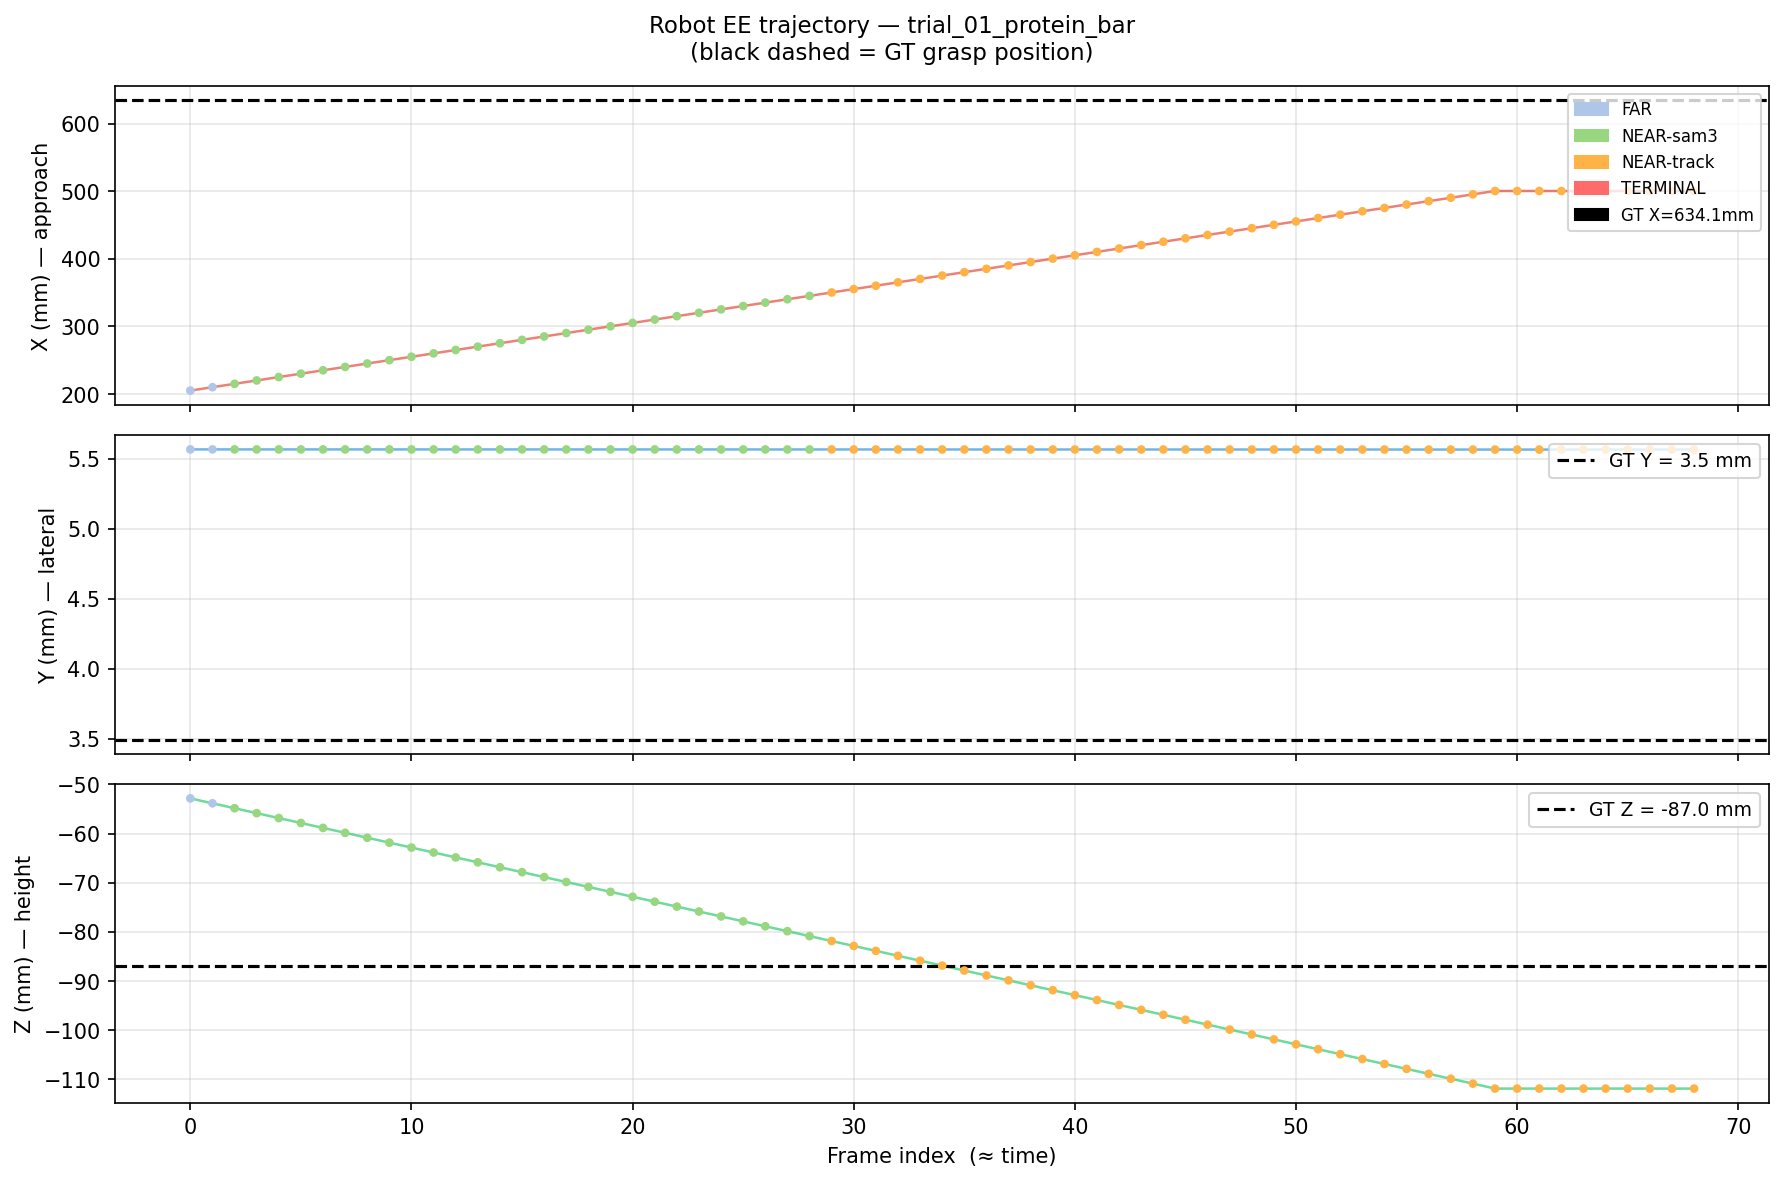
\includegraphics[width=\columnwidth]{figures/robot_xyz_trajectory.png}
  \caption{End-effector trajectory during the pilot trial on the protein-bar
           box.  The robot advanced approximately 295\,mm along the forward
           axis; lateral displacement remained small throughout.}
  \label{fig:robot_traj}
\end{figure}

\subsubsection{Centroid Error Over Time and Depth}

Figure~\ref{fig:centroid_error_frames} shows the pixel-space error
$\lVert\mathbf{e}\rVert_2$ between the estimated target centroid and the
image centre over the course of the trial.  In the early \textsc{near}
phase (frames 3--28, before lock), Signal~E reported centroid errors
between 62.7\,px and 70.0\,px (mean 64.9\,px), reflecting the initial
lateral offset between the robot and the target.  After the lock
transition at frame 29, the fusion estimator combined Signals~A and~B,
with fused centroid errors between 64.7\,px and 162.6\,px (mean
112.0\,px).

Figure~\ref{fig:centroid_error_depth} shows the same centroid error
plotted against stereo depth.  The relationship between approach distance
and error accuracy is a central hypothesis of this work: the system is
expected to improve in precision as the EE approaches the target.  Analysis
of this pilot trial provides a baseline characterisation of this trend,
though the full factorial experiment is required for statistical conclusions.

\begin{figure}[t]
  \centering
  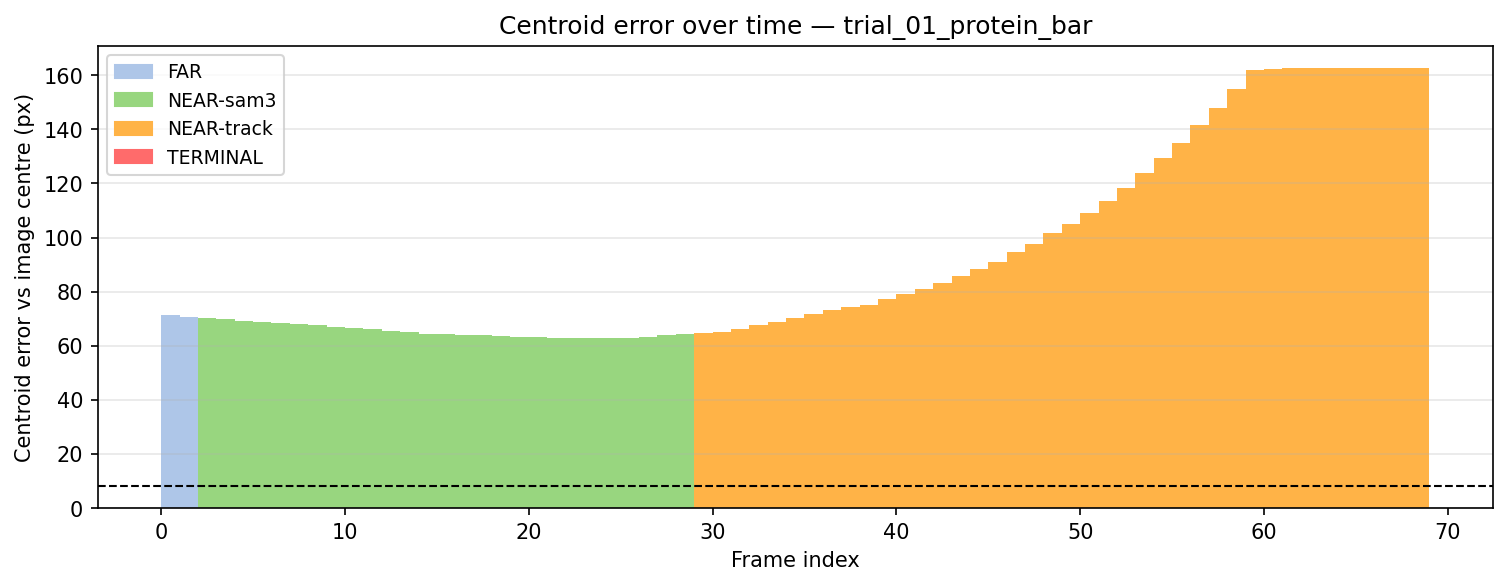
\includegraphics[width=\columnwidth]{figures/centroid_error_over_frames.png}
  \caption{Pixel centroid error $\lVert\mathbf{e}\rVert_2$ versus frame
           index.  The dashed vertical line marks the lock transition at
           frame 29 (depth 317.5\,mm).  Error is measured from the image
           centre to the estimated target centroid.}
  \label{fig:centroid_error_frames}
\end{figure}

\begin{figure}[t]
  \centering
  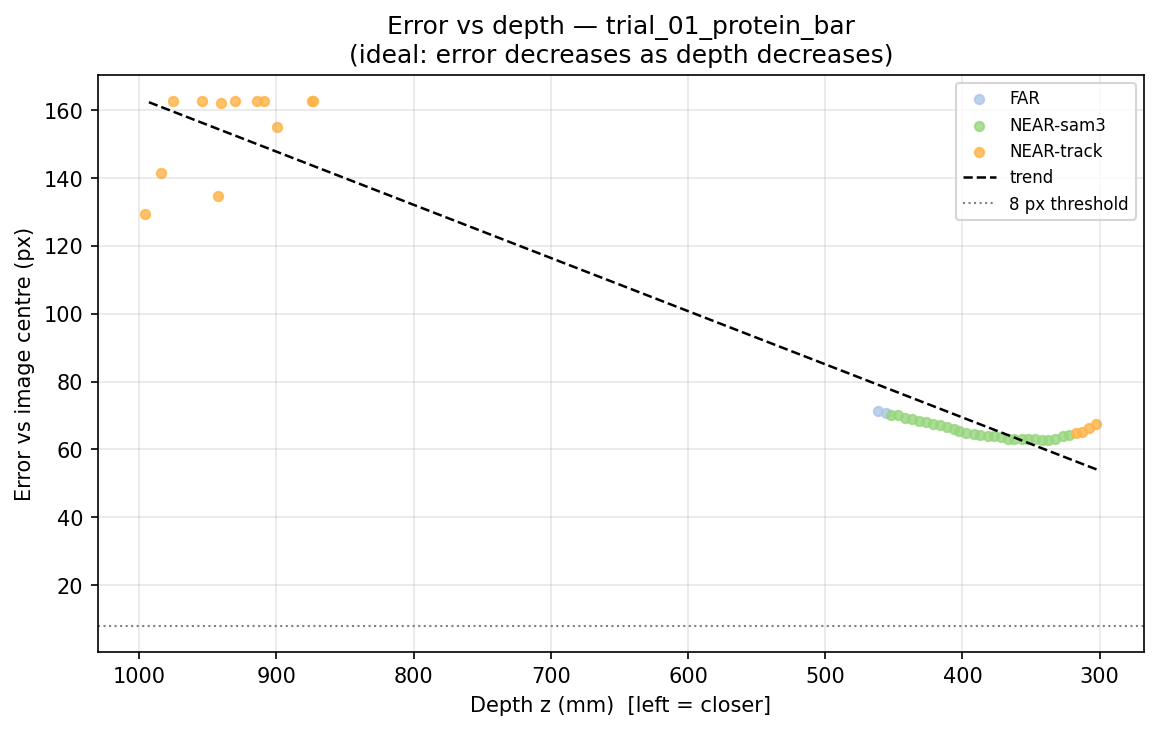
\includegraphics[width=\columnwidth]{figures/centroid_error_vs_depth.png}
  \caption{Centroid error (px) as a function of stereo depth (mm).  The
           plot characterises whether the error signal improves as the
           robot approaches the target.}
  \label{fig:centroid_error_depth}
\end{figure}

\subsubsection{Signal Behaviour in the NEAR Phase}

Figure~\ref{fig:signal_x} and Figure~\ref{fig:signal_y} show the
horizontal and vertical pixel coordinates of each active signal
(Signal~A, Signal~B, Signal~E, and the fused estimate) over the trial
duration.  In frames 29--63, Signal~B (CoTracker3) and Signal~A (locked
3-D reprojection) were both active.  In the later frames (64--68), the
fused estimate followed Signal~B, with weights of $w_B = 1.0$ and
$w_E = 0.0$.  Signal~A placed the reprojected centroid near the left
border of the image at these frames, while Signal~B tracked a location
near the right side.  This divergence between signals in the late
\textsc{near} phase indicates that further investigation is needed into
hand-eye calibration accuracy and CoTracker3 drift over long approach
sequences.

\begin{figure}[t]
  \centering
  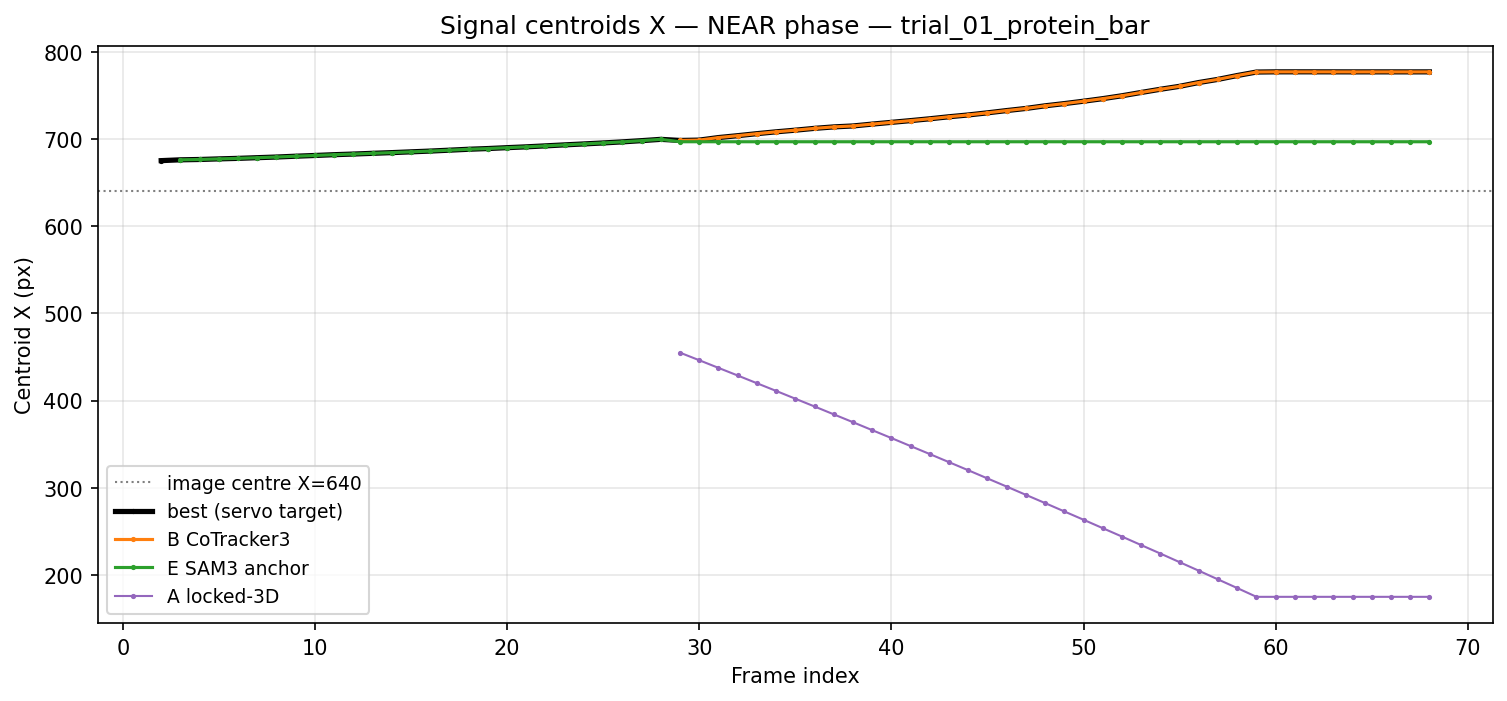
\includegraphics[width=\columnwidth]{figures/signal_centroids_x.png}
  \caption{Horizontal pixel coordinate of each signal's centroid estimate
           over the trial.  Signal~A, Signal~B, Signal~E, and the fused
           estimate are shown separately.  Divergence between signals in
           the late frames suggests tracking drift or calibration error.}
  \label{fig:signal_x}
\end{figure}

\begin{figure}[t]
  \centering
  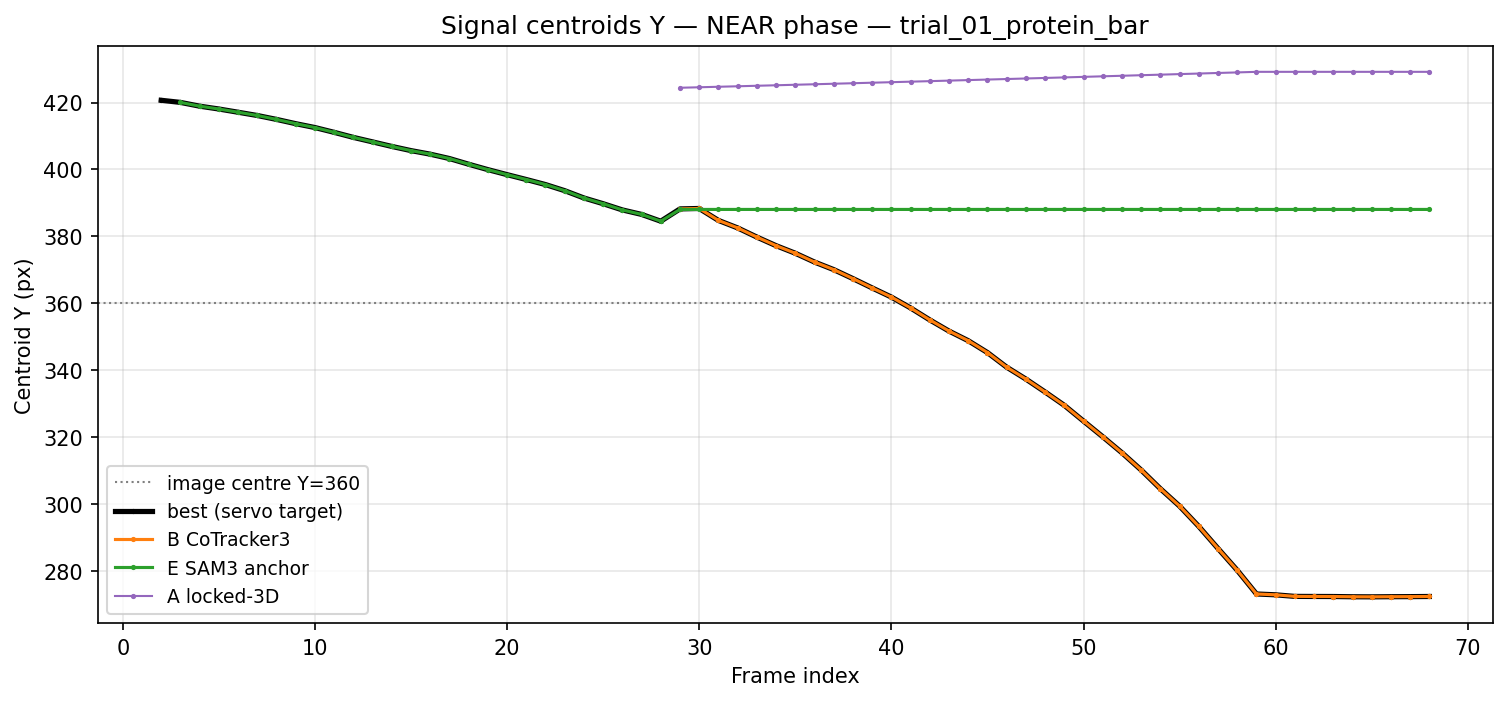
\includegraphics[width=\columnwidth]{figures/signal_centroids_y.png}
  \caption{Vertical pixel coordinate of each signal's centroid estimate
           over the trial (same layout as Figure~\ref{fig:signal_x}).}
  \label{fig:signal_y}
\end{figure}

\subsubsection{Tilt Estimation}

Figure~\ref{fig:tilt_frames} shows the estimated surface tilt angle (in
degrees, from the RANSAC plane fit) over the trial.  In frames 3--32,
tilt remained low (0.33--5.04$^\circ$), consistent with a flat face
presented to the camera.  In frames 52 onward, tilt estimates rose
substantially (28--89$^\circ$), indicating either a genuine angular
misalignment of the target face at closer range or numerical instability
in the RANSAC plane fit when the depth patch contains noisy stereo
measurements.  Figure~\ref{fig:tilt_depth} plots tilt against stereo
depth and shows that the high-tilt regime coincided with shallow stereo
depth readings, supporting the hypothesis of depth-measurement noise at
close range.

\begin{figure}[t]
  \centering
  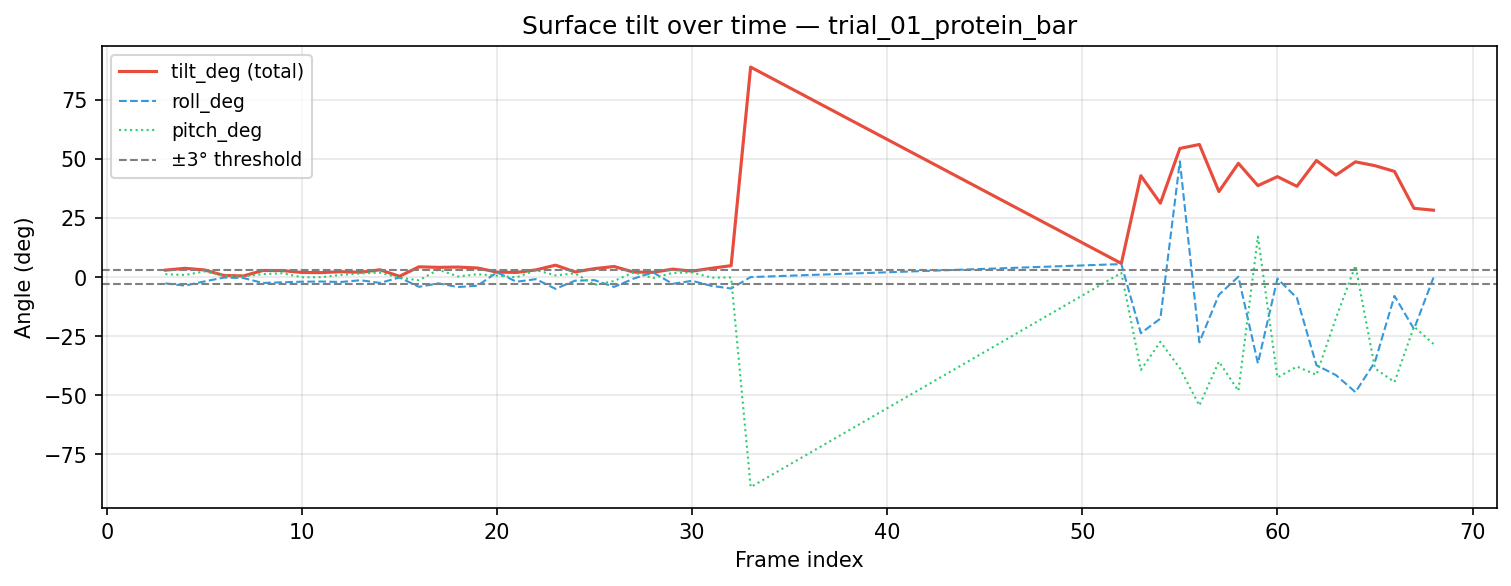
\includegraphics[width=\columnwidth]{figures/tilt_over_frames.png}
  \caption{Estimated surface tilt angle (degrees) versus frame index.
           Low tilt (below 5$^\circ$) in early \textsc{near} frames is
           consistent with a flat face presentation.  High tilt in late
           frames may reflect depth noise at close range.}
  \label{fig:tilt_frames}
\end{figure}

\begin{figure}[t]
  \centering
  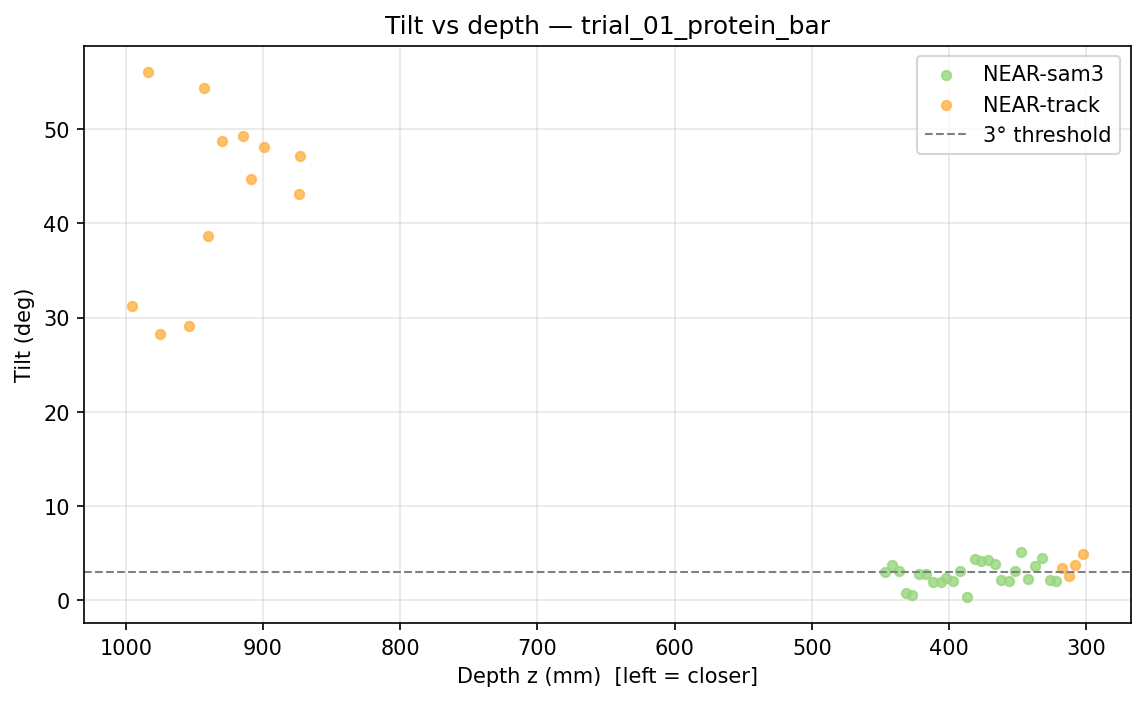
\includegraphics[width=\columnwidth]{figures/tilt_vs_depth.png}
  \caption{Surface tilt angle versus stereo depth.  High tilt
           estimates occur at shallower depths, consistent with increasing
           stereo depth noise at short range.}
  \label{fig:tilt_depth}
\end{figure}

\subsubsection{Phase Timeline}

Figure~\ref{fig:phase_timeline} shows the state machine phase assignment
for each frame alongside the stereo depth reading.  The rapid transition
from \textsc{far} to \textsc{near} after only two frames suggests that
the lock-entry conditions (box area, depth, and border clearance) were
satisfied almost immediately at the starting pose used in this trial.
For future trials, the starting pose should be selected to ensure a
longer \textsc{far}-phase segment that exercises the SAM3-only control
law over a meaningful depth range.

\begin{figure}[t]
  \centering
  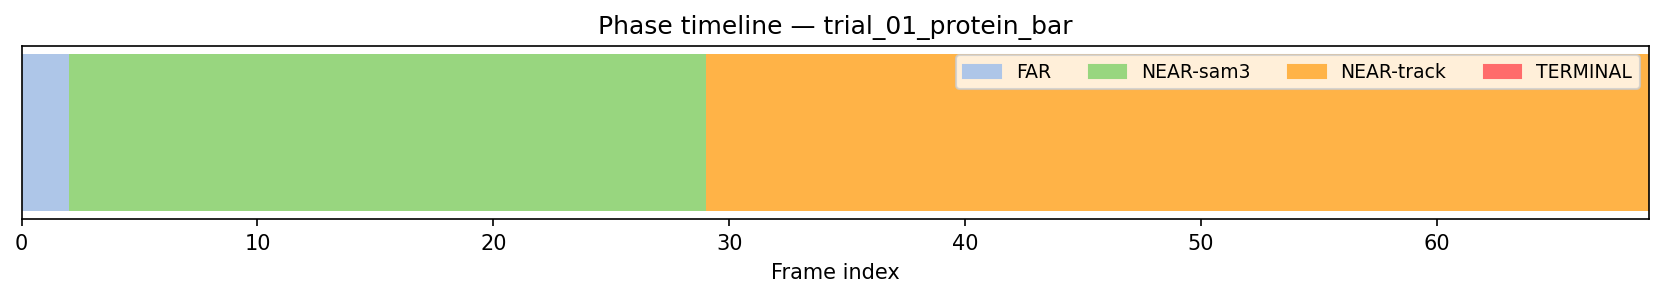
\includegraphics[width=\columnwidth]{figures/phase_timeline.png}
  \caption{State machine phase assignment (top) and stereo depth in mm
           (bottom) versus frame index.  The system transitioned from
           \textsc{far} to \textsc{near} after two frames and remained
           in the \textsc{near} state for the duration of the trial.}
  \label{fig:phase_timeline}
\end{figure}

\subsection{Full Experiment Results (Planned)}
\label{sec:results_full}

Table~\ref{tab:main_results} will report the primary alignment and timing
metrics aggregated over 10 trials per cell (starting poses pooled) once the
full factorial experiment is complete.

\begin{table*}[t]
  \centering
  \caption{Table~I: Servoing Precision Across Box Types and Configurations
           (mean $\pm$ std, $N=10$ per cell, starting poses pooled).
           $\varepsilon_{\text{lat}}$: lateral error (mm);
           $\varepsilon_{\text{depth}}$: depth error (mm);
           $\varepsilon_{3D}$: 3-D Euclidean error (mm);
           $t_{\text{conv}}$: convergence time (s).}
  \label{tab:main_results}
  \begin{tabular}{@{}llcccc@{}}
    \toprule
    Box & Config
      & $\varepsilon_{\text{lat}}$\,(mm)
      & $\varepsilon_{\text{depth}}$\,(mm)
      & $\varepsilon_{3D}$\,(mm)
      & $t_{\text{conv}}$\,(s) \\
    \midrule
    B1 & C1 & ---\,$\pm$\,--- & ---\,$\pm$\,--- & ---\,$\pm$\,--- & ---\,$\pm$\,--- \\
    B1 & C2 & ---\,$\pm$\,--- & ---\,$\pm$\,--- & ---\,$\pm$\,--- & ---\,$\pm$\,--- \\
    B1 & C3 & ---\,$\pm$\,--- & ---\,$\pm$\,--- & ---\,$\pm$\,--- & ---\,$\pm$\,--- \\
    B1 & C4 & ---\,$\pm$\,--- & ---\,$\pm$\,--- & ---\,$\pm$\,--- & ---\,$\pm$\,--- \\
    B2 & C1 & ---\,$\pm$\,--- & ---\,$\pm$\,--- & ---\,$\pm$\,--- & ---\,$\pm$\,--- \\
    B2 & C2 & ---\,$\pm$\,--- & ---\,$\pm$\,--- & ---\,$\pm$\,--- & ---\,$\pm$\,--- \\
    B2 & C3 & ---\,$\pm$\,--- & ---\,$\pm$\,--- & ---\,$\pm$\,--- & ---\,$\pm$\,--- \\
    B2 & C4 & ---\,$\pm$\,--- & ---\,$\pm$\,--- & ---\,$\pm$\,--- & ---\,$\pm$\,--- \\
    B3 & C1 & ---\,$\pm$\,--- & ---\,$\pm$\,--- & ---\,$\pm$\,--- & ---\,$\pm$\,--- \\
    B3 & C2 & ---\,$\pm$\,--- & ---\,$\pm$\,--- & ---\,$\pm$\,--- & ---\,$\pm$\,--- \\
    B3 & C3 & ---\,$\pm$\,--- & ---\,$\pm$\,--- & ---\,$\pm$\,--- & ---\,$\pm$\,--- \\
    B3 & C4 & ---\,$\pm$\,--- & ---\,$\pm$\,--- & ---\,$\pm$\,--- & ---\,$\pm$\,--- \\
    B4 & C1 & ---\,$\pm$\,--- & ---\,$\pm$\,--- & ---\,$\pm$\,--- & ---\,$\pm$\,--- \\
    B4 & C2 & ---\,$\pm$\,--- & ---\,$\pm$\,--- & ---\,$\pm$\,--- & ---\,$\pm$\,--- \\
    B4 & C3 & ---\,$\pm$\,--- & ---\,$\pm$\,--- & ---\,$\pm$\,--- & ---\,$\pm$\,--- \\
    B4 & C4 & ---\,$\pm$\,--- & ---\,$\pm$\,--- & ---\,$\pm$\,--- & ---\,$\pm$\,--- \\
    B5 & C1 & ---\,$\pm$\,--- & ---\,$\pm$\,--- & ---\,$\pm$\,--- & ---\,$\pm$\,--- \\
    B5 & C2 & ---\,$\pm$\,--- & ---\,$\pm$\,--- & ---\,$\pm$\,--- & ---\,$\pm$\,--- \\
    B5 & C3 & ---\,$\pm$\,--- & ---\,$\pm$\,--- & ---\,$\pm$\,--- & ---\,$\pm$\,--- \\
    B5 & C4 & ---\,$\pm$\,--- & ---\,$\pm$\,--- & ---\,$\pm$\,--- & ---\,$\pm$\,--- \\
    \midrule
    ALL & ALL & ---\,$\pm$\,--- & ---\,$\pm$\,--- & ---\,$\pm$\,--- & ---\,$\pm$\,--- \\
    \bottomrule
  \end{tabular}
\end{table*}


% =========================================================================
\section{Discussion}
\label{sec:discussion}

\subsection{Hand-Eye Calibration}

Equations~\eqref{eq:transform} and~\eqref{eq:gt_transform} require the
hand-eye matrix $\mathbf{T}_{\text{ee,cam}}$ relating the ZED Mini optical
frame to the xArm tool-centre-point frame.  This calibration has not yet
been performed.  In the current implementation, $\mathbf{T}_{\text{ee,cam}}$
defaults to the $4\times4$ identity matrix, which is valid only if the
camera frame and tool frame are co-located and co-aligned.  Any physical
offset or rotation of the camera mount introduces a systematic bias in
ground-truth measurements and disables Signal~A in the last-mile fusion.
The divergence of Signal~A from Signal~B observed in the pilot trial
(Figures~\ref{fig:signal_x} and~\ref{fig:signal_y}) is consistent with
this uncalibrated offset.  Hand-eye calibration must be performed before
quantitative 3-D alignment results can be reported.

\subsection{Depth Noise and Tilt Estimation at Close Range}

The RANSAC plane fit used for tilt estimation and TERMINAL-state contact
direction relies on metric stereo depth from the ZED Mini.  At short
standoff distances (below approximately 150\,mm), ZED Mini stereo depth
becomes less reliable due to the limited baseline of the camera.  The
spike in tilt estimates observed beyond frame 52 in the pilot trial is
consistent with this noise floor.  Depth Anything V2 is available as a
fallback depth source, but its output is relative rather than metric and
requires scale calibration before it can substitute for the millimetre-level
thresholds in the state machine.

\subsection{Integration of Far-Range and Last-Mile Phases}

In the current codebase, the SAM3 far-range pipeline and the last-mile
multi-signal fusion pipeline are implemented as separate modules.  The pilot
experiment exercises the integrated path, but the automatic handoff at the
lock transition has not been validated across a wide range of starting
conditions.  In particular, the pilot trial entered the \textsc{near} state
after only two \textsc{far}-state frames, leaving insufficient data to
characterise the SAM3-only control performance at larger standoff distances.

\subsection{Servo Update Rate and SAM3 Latency}

The minimum inter-command interval is $0.3$\,s, giving a maximum control
rate of approximately $3.3$\,Hz.  SAM3 is queried on every camera frame,
meaning that the effective control rate is limited by the SAM3 inference
latency in addition to the $0.3$\,s floor.  Quantifying this latency on
the experimental GPU and assessing whether it imposes a practical bottleneck
relative to the maximum robot speed is a planned measurement.

\subsection{Ground-Truth Error Floor from Manual Alignment}

The ground truth protocol relies on the operator manually jogging the EE
to the face centre of the target box.  The repeatability of this alignment
step is limited by the precision achievable by eye, which is approximately
3--5\,mm.  Any residual error in the manual placement directly biases all
subsequent alignment error measurements: a reported final error of, say,
4\,mm may partly or entirely reflect GT placement error rather than
autonomous servoing error.  Characterising this floor independently---by
repeating the manual jog from the same starting pose multiple times and
measuring the spread of recorded positions---is a prerequisite for
interpreting results at sub-centimetre precision.

\subsection{Robustness Axes Not Yet Evaluated}

The pilot trial used a single box in a controlled single-object environment.
The planned factorial experiment will additionally test: appearance variation
across five box types; background and stack-height configurations;
hard-negative distractors (boxes with similar texture to the target); and
3-D rotation conditions where the visible face is tilted relative to the
approach axis.  None of these conditions have been evaluated quantitatively
at the time of writing.


% =========================================================================
\section{Conclusion}
\label{sec:conclusion}

We have presented a complete visual servoing pipeline for suction-cup grasping
that requires only a single reference image and no task-specific retraining.
The system combines SAM3 open-vocabulary segmentation for far-range approach
with a four-signal fusion estimator---comprising locked-3D reprojection,
CoTracker3 point tracking, a SAM2 watchdog, and DINOv2 feature
matching---to maintain a reliable centroid estimate as the target exits the
camera field of view.  Online Jacobian calibration via optical flow removes
the need for a pre-measured camera-robot mapping, and RANSAC plane fitting on
stereo depth provides surface normal estimates for final contact alignment.

A pilot trial on a protein-bar box validated the end-to-end pipeline over a
296\,mm forward approach.  SAM3 achieved detection confidence above 0.94 on
all 69 frames and ResNet-18 reference similarity above 0.92, demonstrating
that the reference-guided disambiguation reliably identifies the target.  The
state machine transitioned correctly from \textsc{far} to \textsc{near} and
activated the multi-signal fusion estimator.  The pilot also surfaced two
issues that require attention before quantitative claims can be made:
Signal~A (locked-3D reprojection) diverged substantially from Signal~B
(CoTracker3) in the final approach segment, pointing to the need for
hand-eye calibration; and tilt estimates became unreliable at depths below
approximately 150\,mm, consistent with the ZED Mini's stereo noise floor at
close range.

The primary open items are: performing hand-eye calibration to enable
accurate Signal~A and ground-truth 3-D error measurement; characterising
SAM3 inference latency; validating the lock transition across a wider range
of starting conditions; and executing the full factorial experiment (600
trials across five box types, four configurations, and three starting poses)
with the three additional perception backends (GroundingDINO with SAM2,
OWLv2 with SAM2, and DINOv2 feature matching) to quantify the ablation
contribution of each component.  Successful completion of these steps will
determine whether the proposed pipeline achieves the target success rate
across the full set of robustness axes required for the paper's deployment
claim.


% =========================================================================
\section*{Acknowledgments}
I would like to thank Prof.\ Jeffrey Ichnowski for his invaluable guidance,
technical insight, and consistent support throughout this project. His
mentorship at the Momentum Robotics Lab has been central in shaping both the
research direction and the system design presented in this work.
The author also thanks the members of the Momentum Robotics Lab for their
helpful discussions and feedback during development. Access to the xArm
manipulator, ZED Mini stereo camera, and associated lab infrastructure was
essential to the real-world experiments reported here.
This work was carried out as part of an independent study in the Master of
Science in Computer Vision program at Carnegie Mellon University's Robotics
Institute.

\begin{thebibliography}{99}

\bibitem{espiau1992new}
B.~Espiau, F.~Chaumette, and P.~Rives,
``A new approach to visual servoing in robotics,''
\emph{IEEE Trans.\ Robot.\ Autom.}, vol.~8, no.~3, pp.~313--326, 1992.

\bibitem{chaumette2006visual}
F.~Chaumette and S.~Hutchinson,
``Visual servo control. I. Basic approaches,''
\emph{IEEE Robot.\ Autom.\ Mag.}, vol.~13, no.~4, pp.~82--90, 2006.

\bibitem{chaumette2007visual}
F.~Chaumette and S.~Hutchinson,
``Visual servo control. II. Advanced approaches,''
\emph{IEEE Robot.\ Autom.\ Mag.}, vol.~14, no.~1, pp.~109--118, 2007.

\bibitem{piepmeier2004uncalibrated}
J.~A.~Piepmeier, G.~V.~McMurray, and H.~Lipkin,
``Uncalibrated dynamic visual servoing,''
\emph{IEEE Trans.\ Robot.\ Autom.}, vol.~20, no.~1, pp.~143--147, 2004.

\bibitem{bateux2017training}
Q.~Bateux and E.~Marchand,
``Training deep neural networks for visual servoing,''
in \emph{Proc.\ IEEE Int.\ Conf.\ Robot.\ Autom.}, 2017, pp.~3307--3314.

\bibitem{saxena2017neural}
A.~Saxena, H.~Driess, and M.~Toussaint,
``Neural task programming: Learning to generalize across hierarchical tasks,''
in \emph{Proc.\ IEEE Int.\ Conf.\ Robot.\ Autom.}, 2018.

\bibitem{lampe2023learning}
T.~Lampe \emph{et al.},
``Learning visual servoing with deep features and fitted Q-iteration,''
in \emph{Proc.\ ICLR}, 2023.

\bibitem{kirillov2023segment}
A.~Kirillov \emph{et al.},
``Segment anything,''
in \emph{Proc.\ IEEE/CVF ICCV}, 2023, pp.~4015--4026.

\bibitem{ravi2024sam2}
N.~Ravi \emph{et al.},
``SAM 2: Segment anything in images and videos,''
\emph{arXiv:2408.00714}, 2024.

\bibitem{liu2023grounding}
S.~Liu \emph{et al.},
``Grounding DINO: Marrying DINO with grounded pre-training for open-set
object detection,''
\emph{arXiv:2303.05499}, 2023.

\bibitem{minderer2023scaling}
M.~Minderer \emph{et al.},
``Scaling open-vocabulary object detection,''
in \emph{Proc.\ NeurIPS}, 2023.

\bibitem{liu2024graspgdino}
W.~Liu \emph{et al.},
``Open-vocabulary grasping detection using GroundingDINO,''
\emph{arXiv}, 2024.

\bibitem{tang2023taskgrasp}
H.~Tang \emph{et al.},
``TaskGrasp: Multi-object, multi-task generalizable robot grasping,''
in \emph{Proc.\ CoRL}, 2023.

\bibitem{oquab2023dinov2}
M.~Oquab \emph{et al.},
``DINOv2: Learning robust visual features without supervision,''
\emph{arXiv:2304.07193}, 2023.

\bibitem{amir2022deep}
S.~Amir \emph{et al.},
``Deep spectral methods: A surprisingly strong baseline for unsupervised
semantic segmentation and localization,''
in \emph{Proc.\ IEEE/CVF CVPR}, 2022.

\bibitem{karaev2024cotracker3}
N.~Karaev \emph{et al.},
``CoTracker3: Simpler and better point tracking by pseudo-labelling real
videos,''
\emph{arXiv:2410.11831}, 2024.

\bibitem{yoshimi1994active}
B.~H.~Yoshimi and P.~K.~Allen,
``Active, uncalibrated visual servoing,''
in \emph{Proc.\ IEEE Int.\ Conf.\ Robot.\ Autom.}, 1994, pp.~156--161.

\bibitem{mahler2017dex}
J.~Mahler \emph{et al.},
``Dex-Net 2.0: Deep learning to plan robust grasps with synthetic point
clouds and analytic grasp metrics,''
in \emph{Proc.\ RSS}, 2017.

\bibitem{mahler2019learning}
J.~Mahler \emph{et al.},
``Learning ambidextrous robot grasping policies,''
\emph{Sci.\ Robot.}, vol.~4, no.~26, 2019.

\end{thebibliography}

\vfill

\end{document}
